\normalfalse \difficiletrue \tdifficilefalse
\correctionfalse

%\UPSTIidClasse{11} % 11 sup, 12 spé
%\newcommand{\UPSTIidClasse}{12}

\exer{Barrière Sympact $\star\star$ \label{B2:12:14}}
\setcounter{question}{0}\UPSTIcompetence{B2-12}
\index{Compétence B2-12}
\index{Barrière Sympact}
\ifcorrection
\else
\marginnote{\textbf{Pas de corrigé pour cet exercice.}}
\fi
\ifprof
\else
Soit le mécanisme suivant. On a $\vect{AC}=H\vect{j_0}$ et $\vect{CB}=R\vect{i_1}$. De plus, 
$H=\SI{120}{mm}$, $R=\SI{40}{mm}$ $BI=\SI{10}{mm}$.

\begin{center}
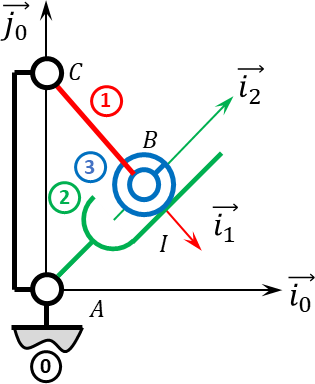
\includegraphics[width=\linewidth]{15_01}
\end{center}
\fi

\question{Tracer le graphe des liaisons.}
\ifprof
\else
\fi

\question{Retracer le schéma cinématique pour $\theta(t)=\dfrac{\pi}{2}\,\text{rad}$.}
\ifprof
\else
\fi

\question{Retracer le schéma cinématique pour $\theta(t)=-\dfrac{\pi}{2}\,\text{rad}$.}
\ifprof
\else
\fi


%\question{En déduire la course de la pièce \textbf{3}.}
%\ifprof
%\else
%\fi



\ifprof
\else
\begin{flushright}
\footnotesize{Corrigé  voir \ref{B2:12:14}.}
\end{flushright}%
\fi